%% ============================================================================
%% architecture.tex -- README architecture figure, biomimetic-lattice-pipeline
%%
%% Purpose : module-level view of the pipeline, drawn in the same visual language
%%           as the README overview and the sister packages' figures (grey page,
%%           gold icon rings, navy stage boxes, gold module tags) so the figures
%%           read as one set. Seven stages run left to right, and each names the
%%           package module that implements it. The dashed gold path above them is
%%           the Optuna closed loop (orchestration/optimize.py, closed_loop.py):
%%           it proposes new CAD parameters, re-runs the build-solve-score chain,
%%           and reverse-maps the best designs back to biology.
%%           It replaces the matplotlib box diagram 01_architecture.png in the
%%           README; that PNG and its generator stay, because docs/PIPELINE.tex
%%           still includes it.
%% Build   : (from docs/figures/src/)
%%           pdflatex architecture.tex
%%           pdftoppm -png -r 254 -singlefile architecture.pdf ../architecture
%% Output  : a 28 cm x 11.1 cm vector PDF; at 254 dpi the PNG is 2800 px wide.
%%           GitHub shows it ~830-1000 px wide, so the 14.5 pt box labels land
%%           near 15-18 px and the 11 pt captions near 11-14 px on screen.
%% Layout  : rows are fixed y-bands (loop, icon rings, boxes, captions, footer)
%%           and the seven columns sit at fixed x-centres 3.8 cm apart, so no
%%           text can collide with an icon or a neighbouring caption.
%% ============================================================================
\documentclass[tikz,border=0pt]{standalone}
\usepackage[T1]{fontenc}
\usepackage{lmodern}                      % scalable tt/math fonts (no bitmap substitutions)
\usepackage[scaled=0.95]{helvet}          % Helvetica metrics, like the sister figures
\renewcommand{\familydefault}{\sfdefault}
\usetikzlibrary{arrows.meta,calc}
\pdfinfo{/Title (biomimetic-lattice-pipeline: architecture) /Author (Cameron B. Renteria)}

% ---- palette: identical hex values to the overview and the sister packages -------------
\definecolor{page}{HTML}{EEEEEE}    % page grey
\definecolor{navy}{HTML}{1E3252}    % stage boxes, line icons, arrows
\definecolor{gold}{HTML}{B8894A}    % icon rings, module tags, the optimization loop
\definecolor{ink}{HTML}{222222}     % caption text
\definecolor{tone}{HTML}{C9CED6}    % neutral fill inside icons

% ---- reusable styles --------------------------------------------------------------------
\tikzset{
  % Navy stage box: two-line plain-English stage name in white.
  stage/.style = {fill=navy, rounded corners=6pt, minimum width=3.3cm, minimum height=1.6cm,
                  text width=3.1cm, text=white, align=center,
                  font=\fontsize{14.5}{17}\selectfont, inner sep=2pt},
  % Gold icon ring above each box (radius 1.05 cm); the glyph inside stays within +-0.65 cm.
  ring/.style  = {draw=gold, line width=1.6pt, circle, minimum size=2.1cm},
  % Caption under each box: gold module tag on the first line, then a short description.
  capt/.style  = {text=ink, align=center, anchor=north, text width=3.55cm,
                  font=\fontsize{11}{13.4}\selectfont,
                  execute at begin node={\hyphenpenalty=10000\exhyphenpenalty=10000}},
  % Forward data flow between stages.
  flow/.style  = {-{Stealth[length=6pt,width=6pt]}, line width=1.3pt, draw=navy},
  % Line work of the icons.
  ico/.style   = {draw=navy, line width=1.1pt, line cap=round, line join=round},
  % The Optuna closed loop: dashed gold, with a page-grey halo so it reads cleanly.
  loop/.style  = {draw=gold, line width=1.4pt, dash pattern=on 5pt off 3.5pt,
                  -{Stealth[length=7pt,width=6.5pt]}},
}
% Module tag: gold monospace, set as the first caption line (as in the SOM figure).
\newcommand{\tagline}[1]{{\color{gold}\ttfamily\fontsize{10.5}{13}\selectfont #1}}

\begin{document}
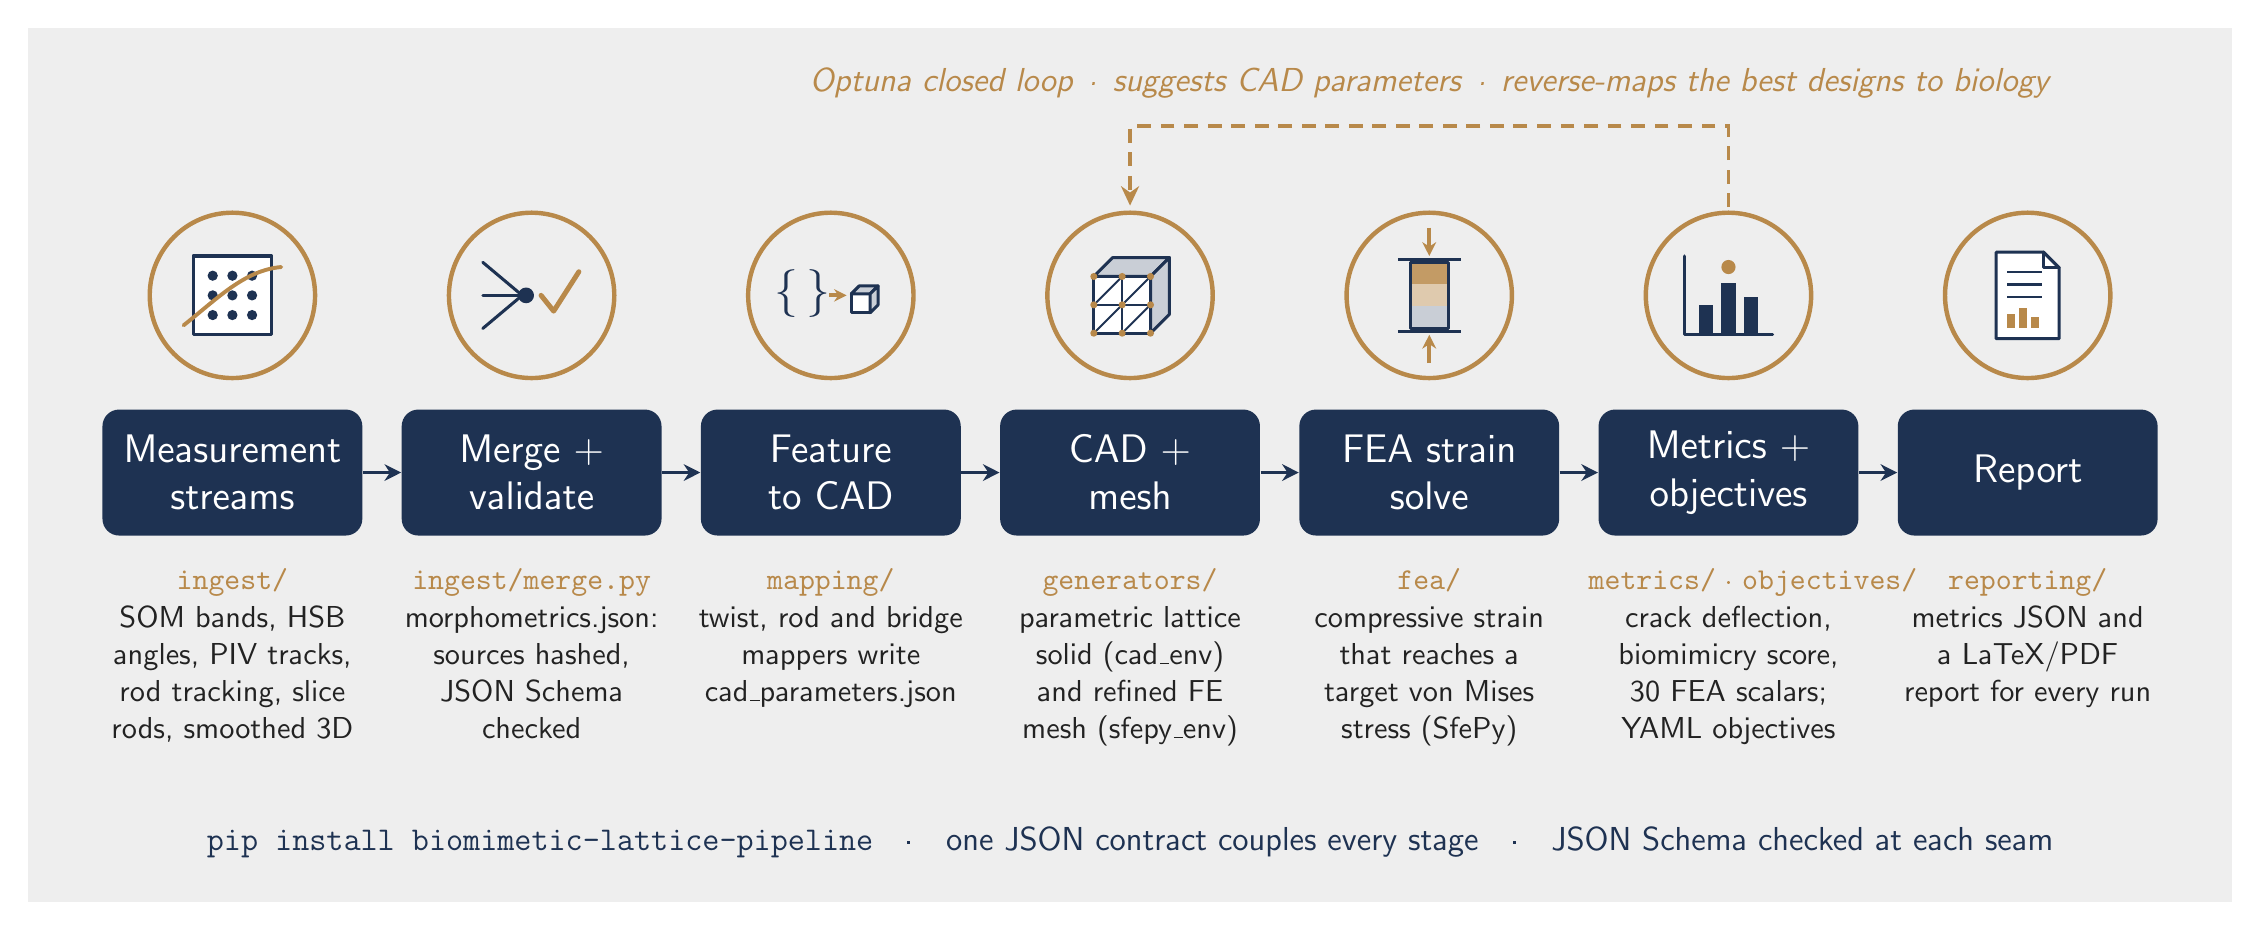
\begin{tikzpicture}[x=1cm,y=1cm]

% ---- page -------------------------------------------------------------------------------
\fill[page] (0,0.9) rectangle (28,12);   % bottom edge at 0.9: footer sits ~1 cm under the captions

% ---- column centres (x) and fixed row bands (y) -------------------------------------------
%  measure 2.6 | merge 6.4 | map 10.2 | build 14.0 | solve 17.8 | score 21.6 | report 25.4
\def\yloop{10.75}  % horizontal run of the Optuna loop
\def\yring{8.6}    % icon ring centres (ring spans 7.55-9.65)
\def\ybox{6.35}    % stage box centres (box spans 5.55-7.15)
\def\ycap{5.25}    % caption tops

% ---- icon rings ---------------------------------------------------------------------------
\foreach \x in {2.6,6.4,10.2,14.0,17.8,21.6,25.4} \node[ring] at (\x,\yring) {};

% Icon 1 -- measurement streams: a micro-CT slice of rod cross-sections with one gold
% rod trajectory through it (the tracked, segmented and SOM-banded measurements).
\begin{scope}[shift={(2.6,\yring)}]
  \draw[ico, fill=white] (-0.5,-0.5) rectangle (0.5,0.5);
  \foreach \i in {-0.25,0,0.25} \foreach \j in {-0.25,0,0.25}
    \fill[navy] (\i,\j) circle (0.065);
  \draw[gold, line width=1.4pt, line cap=round]
    (-0.62,-0.38) .. controls (-0.2,-0.05) and (0.15,0.32) .. (0.62,0.36);
\end{scope}

% Icon 2 -- merge + validate: three sources converge on one record, then a gold check
% (JSON Schema validation of the merged morphometrics.json).
\begin{scope}[shift={(6.4,\yring)}]
  \draw[ico] (-0.62,0.42) -- (-0.12,0.0);
  \draw[ico] (-0.62,0.0)  -- (-0.12,0.0);
  \draw[ico] (-0.62,-0.42) -- (-0.12,0.0);
  \fill[navy] (-0.07,0.0) circle (0.1);
  \draw[gold, line width=1.8pt, line cap=round, line join=round]
    (0.12,0.0) -- (0.28,-0.2) -- (0.6,0.3);
\end{scope}

% Icon 3 -- feature to CAD: a JSON contract (braces) feeding a gold arrow into a solid.
\begin{scope}[shift={(10.2,\yring)}]
  \node[text=navy, font=\fontsize{19}{19}\selectfont\ttfamily\bfseries] at (-0.36,0.02) {\{\,\}};
  \draw[gold, line width=1.4pt, -{Stealth[length=4.5pt,width=4.5pt]}] (-0.02,0) -- (0.2,0);
  % small isometric cube: front face, top face, right face
  \draw[ico, fill=white] (0.26,-0.22) rectangle (0.5,0.02);
  \draw[ico, fill=tone]  (0.26,0.02) -- (0.36,0.12) -- (0.6,0.12) -- (0.5,0.02) -- cycle;
  \draw[ico, fill=tone]  (0.5,-0.22) -- (0.6,-0.12) -- (0.6,0.12) -- (0.5,0.02) -- cycle;
\end{scope}

% Icon 4 -- CAD + mesh: an isometric solid whose front face is triangulated (the FE mesh);
% gold nodes mark the mesh vertices.
\begin{scope}[shift={(14.0,\yring)}]
  \draw[ico, fill=tone] (-0.46,0.24) -- (-0.22,0.48) -- (0.5,0.48) -- (0.26,0.24) -- cycle;  % top
  \draw[ico, fill=tone] (0.26,-0.48) -- (0.5,-0.24) -- (0.5,0.48) -- (0.26,0.24) -- cycle;   % right
  \draw[ico, fill=white] (-0.46,-0.48) rectangle (0.26,0.24);                                % front
  \draw[navy, line width=0.7pt] (-0.1,-0.48) -- (-0.1,0.24) (-0.46,-0.12) -- (0.26,-0.12);   % grid
  \draw[navy, line width=0.7pt] (-0.46,-0.48) -- (0.26,0.24) (-0.46,-0.12) -- (-0.1,0.24)
                                (-0.1,-0.48) -- (0.26,-0.12);                                % diagonals
  \foreach \p in {(-0.46,-0.48),(-0.1,-0.48),(0.26,-0.48),(-0.46,-0.12),(-0.1,-0.12),
                  (0.26,-0.12),(-0.46,0.24),(-0.1,0.24),(0.26,0.24)}
    \fill[gold] \p circle (0.045);
\end{scope}

% Icon 5 -- FEA strain solve: a specimen under gold compression arrows, banded like a
% stress contour (darker band = higher von Mises stress).
\begin{scope}[shift={(17.8,\yring)}]
  \fill[tone]     (-0.24,-0.42) rectangle (0.24,-0.14);
  \fill[gold!45]  (-0.24,-0.14) rectangle (0.24,0.14);
  \fill[gold!85]  (-0.24,0.14)  rectangle (0.24,0.42);
  \draw[ico] (-0.24,-0.42) rectangle (0.24,0.42);
  \draw[gold, line width=1.5pt, -{Stealth[length=5pt,width=5pt]}] (0,0.86) -- (0,0.5);
  \draw[gold, line width=1.5pt, -{Stealth[length=5pt,width=5pt]}] (0,-0.86) -- (0,-0.5);
  \draw[navy, line width=1.1pt] (-0.4,0.46) -- (0.4,0.46) (-0.4,-0.46) -- (0.4,-0.46);     % platens
\end{scope}

% Icon 6 -- metrics + objectives: three metric bars on axes, the best design marked gold.
\begin{scope}[shift={(21.6,\yring)}]
  \draw[ico] (-0.56,0.5) -- (-0.56,-0.5) -- (0.56,-0.5);
  \fill[navy] (-0.38,-0.5) rectangle (-0.2,-0.12);
  \fill[navy] (-0.09,-0.5) rectangle (0.09,0.16);
  \fill[navy] (0.2,-0.5)   rectangle (0.38,-0.02);
  \fill[gold] (0,0.36) circle (0.09);
\end{scope}

% Icon 7 -- report: a page with text lines and a small gold chart.
\begin{scope}[shift={(25.4,\yring)}]
  \draw[ico, fill=white] (-0.4,-0.55) -- (-0.4,0.55) -- (0.2,0.55) -- (0.4,0.35) -- (0.4,-0.55) -- cycle;
  \draw[ico] (0.2,0.55) -- (0.2,0.35) -- (0.4,0.35);                                          % folded corner
  \foreach \y in {0.3,0.14,-0.02} \draw[navy, line width=0.9pt] (-0.26,\y) -- (0.18,\y);
  \fill[gold] (-0.26,-0.42) rectangle (-0.16,-0.24);
  \fill[gold] (-0.11,-0.42) rectangle (-0.01,-0.16);
  \fill[gold] (0.04,-0.42)  rectangle (0.14,-0.28);
\end{scope}

% ---- stage boxes ----------------------------------------------------------------------------
\node[stage] (s1) at (2.6,\ybox)  {Measurement\\streams};
\node[stage] (s2) at (6.4,\ybox)  {Merge +\\validate};
\node[stage] (s3) at (10.2,\ybox) {Feature\\to CAD};
\node[stage] (s4) at (14.0,\ybox) {CAD +\\mesh};
\node[stage] (s5) at (17.8,\ybox) {FEA strain\\solve};
\node[stage] (s6) at (21.6,\ybox) {Metrics +\\objectives};
\node[stage] (s7) at (25.4,\ybox) {Report};

% ---- forward data flow ------------------------------------------------------------------------
\foreach \a/\b in {s1/s2,s2/s3,s3/s4,s4/s5,s5/s6,s6/s7} \draw[flow] (\a.east) -- (\b.west);

% ---- captions: module tag (gold) + what the stage does -----------------------------------
\node[capt] at (2.6,\ycap)  {\tagline{ingest/}\\SOM bands, HSB angles, PIV tracks, rod tracking, slice rods, smoothed 3D};
\node[capt] at (6.4,\ycap)  {\tagline{ingest/merge.py}\\morphometrics.json: sources hashed, JSON Schema checked};
\node[capt] at (10.2,\ycap) {\tagline{mapping/}\\twist, rod and bridge mappers write cad\_parameters.json};
\node[capt] at (14.0,\ycap) {\tagline{generators/}\\parametric lattice solid (cad\_env) and refined FE mesh (sfepy\_env)};
\node[capt] at (17.8,\ycap) {\tagline{fea/}\\compressive strain that reaches a target von Mises stress (SfePy)};
\node[capt] at (21.6,\ycap) {\tagline{metrics/\,\textperiodcentered\,objectives/}\\crack deflection, biomimicry score, 30 FEA scalars; YAML objectives};
\node[capt] at (25.4,\ycap) {\tagline{reporting/}\\metrics JSON and a LaTeX/PDF report for every run};

% ---- Optuna closed loop: score -> new CAD parameters (drawn last, over everything) ---------
\draw[loop] (21.6,9.72) -- (21.6,\yloop) -- (14.0,\yloop) -- (14.0,9.74);
\node[text=gold, font=\fontsize{12.5}{15}\selectfont\itshape] at (17.8,11.3)
  {Optuna closed loop \,\textperiodcentered\, suggests CAD parameters \,\textperiodcentered\, reverse-maps the best designs to biology};

% ---- footer ---------------------------------------------------------------------------------
\node[text=navy, font=\fontsize{12.5}{15}\selectfont] at (14.0,1.65)
  {\texttt{pip install biomimetic-lattice-pipeline}\quad\textperiodcentered\quad
   one JSON contract couples every stage\quad\textperiodcentered\quad
   JSON Schema checked at each seam};

\end{tikzpicture}
\end{document}
